Throughout the input specification the user is defining variables. As described in the above sections many of these variables can be specified by the user to be random variables with a distribution on their values. It is in the UQ panel that the user specifies what these distributions are. 
It is also here that the user specifies the UQ method and the input values are for these UQ methods. 
The panel is split,  as shown in \autoref{fig:figure10}, into 2 frames:
 \begin{enumerate}
\item Sampling Methods 
\item Random Variables
\end{enumerate}

\begin{figure}[!htbp]
  \centering {
    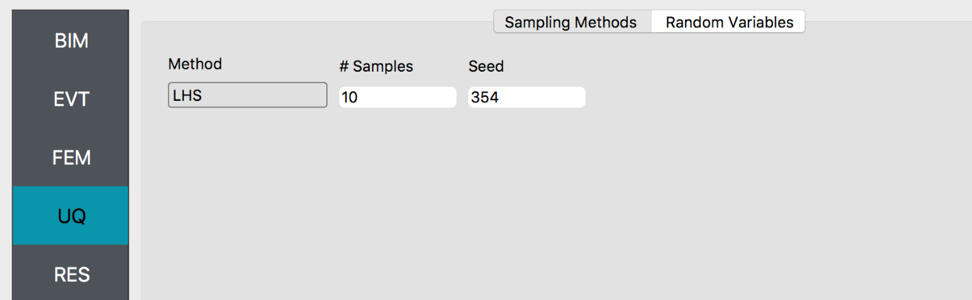
\includegraphics[width=0.8\textwidth]
    {figs/Figure10.png} }
  \caption{UQ}
  \label{fig:figure10}
\end{figure}


\subsection{Sampling Methods}
In the sampling methods the user selects the sampling method to use from the method dropdown. Currently this is limited to two options: 
Monte Carlo and Latin Hypercube Sampling (LHS). For the one selected, the user specifies the number of simulations to be perform and the seed.

\subsection{Random Variables}
The Random Variable panel is where the user enters the random variables. Each random variable has a name and a distribution. The distribution is selected frm the drop-down menu. By changing the distribution type, the inputs required to define the distribution change. The following are the list of distributions available:
\begin{enumerate}
\item Normal
\item Lognormal
\item Beta
\item Uniform
\item Weibull
|item Gumbell
\item UserDef
\end{enumerate} 

As with other panels, the random variables can be added or removed. Care must be taken by the user in ensuring that if the user removes random variables from this panel that they also remove them from the other input widgets. Failing to do so may result in the program faling to complete.


\begin{figure}[!htbp]
  \centering {
    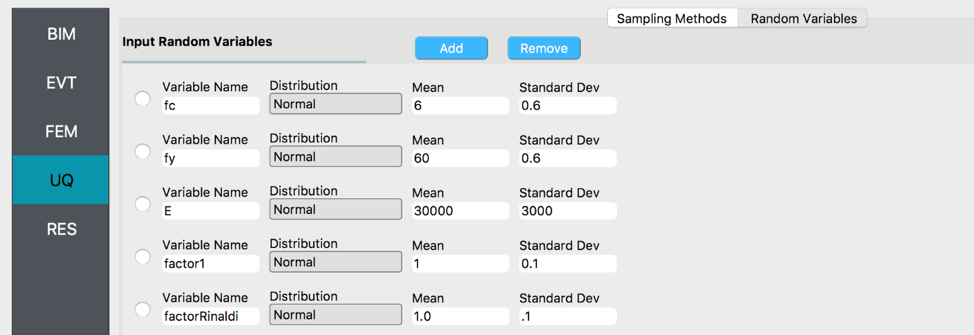
\includegraphics[width=0.8\textwidth]
    {figs/Figure11.png} }
  \caption{Random variables}
  \label{fig:figure11}
\end{figure}
